%==============================================================================
%  Factorize, Don't Truncate  —  low-rank, physics-aware leakage-minimizing
%  dataset splitting.  Landscape 42in x 36in research poster (beamerposter).
%  Compile:  pdflatex lowrank_poster.tex   (run twice)
%
%  Sections: Motivation | Key idea | Leakage metric | Pipeline |
%            Preliminary results | Physics-aware UMA embeddings | Discussion
%==============================================================================
\documentclass[final]{beamer}
\usepackage[orientation=landscape, size=custom,
            width=106.68, height=91.44, scale=1.10]{beamerposter}  % 42in x 36in
\usepackage[T1]{fontenc}
\usepackage[utf8]{inputenc}
\usepackage{helvet}
\renewcommand{\familydefault}{\sfdefault}
\usefonttheme{professionalfonts}
\usepackage{amsmath, amssymb}
\usepackage{graphicx}
\usepackage{tikz}
\usepackage{qrcode}
\usepackage{booktabs}
\usepackage{array}
\usepackage{pifont}
\usepackage{colortbl}
\usetikzlibrary{arrows.meta, positioning, shapes.geometric, calc, fit, backgrounds}
\graphicspath{{figures/}{assets/}}
\setbeamertemplate{navigation symbols}{}

%---- palette ---------------------------------------------------------------
\definecolor{maroon}{HTML}{7A0C00}   % UChicago header maroon
\definecolor{ink}{HTML}{14243B}      % body text
\definecolor{blue}{HTML}{2563EB}     % hero / low-rank
\definecolor{green}{HTML}{1B7A3D}
\definecolor{orange}{HTML}{E8710A}
\definecolor{soft}{HTML}{F3F0EC}     % warm off-white block tint
\definecolor{softblue}{HTML}{EAF1FE}
\definecolor{rulec}{HTML}{D9C7C2}    % soft maroon-tinted rule
\definecolor{gray}{HTML}{5B6472}

\setbeamercolor{background canvas}{bg=white}
\setbeamercolor{normal text}{fg=ink}
\usebeamercolor[fg]{normal text}

%---- section-header macro (centered maroon title + rule) -------------------
%  extra leading above the title so headers never crowd the preceding caption
\newcommand{\pblock}[1]{%
  \par\vspace{1.6ex}%
  \begin{center}{\color{maroon}\bfseries\Large #1}\end{center}%
  \vspace{-1.0ex}{\color{rulec}\rule{\linewidth}{1.3pt}}\par\vspace{0.6ex}}

% tinted callout box
\newcommand{\callout}[2]{%
  \begin{center}\colorbox{#1}{\begin{minipage}{0.93\linewidth}\vspace{0.5ex}
  #2\vspace{0.5ex}\end{minipage}}\end{center}}

\newcommand{\vrulecol}{\begin{column}{0.008\paperwidth}\centering
  {\color{rulec}\rule{1.6pt}{63.5cm}}\end{column}}

\setbeamertemplate{itemize items}[circle]
\setbeamercolor{itemize item}{fg=maroon}
\setbeamercolor{itemize subitem}{fg=maroon}

\begin{document}
\begin{frame}[t]{}

%============================== HEADER (full-bleed) =========================
\begin{tikzpicture}[remember picture, overlay]
  \fill[maroon] (current page.north west) rectangle
        ([yshift=-15.2cm]current page.north east);
  % palm logo (left)
  \node[anchor=west] at ([xshift=2.6cm, yshift=-7.4cm]current page.north west)
        {
\includegraphics[height=12.4cm]{palm_logo}};
  % title block (center) -- constrained width so it never runs under the QR
  \node[anchor=center, text=white, align=center, text width=66cm]
        at ([yshift=-7.0cm]current page.north) {%
    {\fontsize{100}{108}\selectfont\bfseries Factorize, Don't Truncate}\\[10pt]
    {\fontsize{38}{46}\selectfont Physics-aware, graph-free leakage-minimizing
     dataset splitting at 10-million-molecule scale}\\[18pt]
    {\fontsize{33}{39}\selectfont Ruijie Zhu\textsuperscript{1,2},\ \
     Rodrigo Ferreira\textsuperscript{1,3},\ \ Rui Ding\textsuperscript{1,3},\ \
     Haihui Pu\textsuperscript{1,3},\ \ Yuxin Chen\textsuperscript{4},\ \
     Junhong Chen\textsuperscript{1,3}}\\[8pt]
    {\fontsize{23}{29}\selectfont\itshape
     \textsuperscript{1}Pritzker School of Molecular Engineering, University of Chicago;\ \
     \textsuperscript{2}Data Science and Learning Division, Argonne;\ \
     \textsuperscript{3}Chemical Sciences and Engineering, Argonne National Laboratory;\ \
     \textsuperscript{4}Department of Computer Science, University of Chicago}};
  % QR + NSF (right)
  \node[anchor=east, fill=white, inner sep=7pt, rounded corners=5pt]
        (qr) at ([xshift=-2.6cm, yshift=-6.6cm]current page.north east)
        {\qrcode[height=6.4cm, level=M]{https://github.com/Ray16/PALM}};
  \node[anchor=north, text=white, font=\footnotesize\bfseries]
        at ([yshift=-0.2cm]qr.south) {github.com/Ray16/PALM};
  \node[anchor=east] at ([xshift=-16.8cm, yshift=-7.4cm]current page.north east)
        {
\includegraphics[height=8.6cm]{nsf_logo}};
\end{tikzpicture}

%============================== FOOTER (full-bleed band) ====================
\begin{tikzpicture}[remember picture, overlay,
    stat/.style={anchor=center, align=center, text=ink}]
  \fill[soft] ([yshift=6.3cm]current page.south west) rectangle
        (current page.south east);
  \fill[maroon] ([yshift=6.3cm]current page.south west) rectangle
        ([yshift=6.55cm]current page.south east);
  \def\sy{3.05cm}
  \foreach \sx/\sv/\sl [count=\i] in {%
     0.135/{27\,s}/{split the full \textbf{9.55M}-molecule OMol25},
     0.375/{2054$\times$}/{faster than DataSAIL (GPU vs.\ CPU ILP)},
     0.625/{11\,/\,11}/{lowest $L(\pi)$ of the fast splitters, exact 80/20},
     0.865/{exact 80/20}/{every split, exact target ratios}}{
    \node[stat] at ([xshift=\sx\paperwidth, yshift=\sy]current page.south west)
      {{\fontsize{62}{66}\selectfont\bfseries\color{blue}\sv}\\[5pt]
       {\fontsize{26}{32}\selectfont\sl}};
    \ifnum\i<4
      \node at ([xshift={(\sx+0.12)*\paperwidth}, yshift=\sy]current page.south west)
        {\color{rulec}\rule{1.4pt}{4.1cm}};
    \fi}
\end{tikzpicture}

%============================== BODY (3 columns) ============================
\begin{tikzpicture}[remember picture, overlay]
\node[anchor=north west, inner sep=0]
      at ([xshift=2.0cm, yshift=-15.7cm]current page.north west) {%
\begin{minipage}{102.6cm}
%------------------------------- COLUMN 1 ----------------------------------
\begin{minipage}[t]{0.313\linewidth}

\pblock{Motivation}
{\large\textbf{Data leakage inflates ML metrics.} Split a dataset carelessly and
near-duplicates land on both sides. The model then scores by \emph{recall}, not
by \emph{generalization} — the benchmark rewards memorization, and the gap only
surfaces on genuinely new chemistry.}
\vspace{0.6ex}

{\large\textbf{Existing splitters cannot handle large datasets.}}
\begin{itemize}\setlength\itemsep{3pt}\large
  \item \textbf{Exact methods} solve an $O(n^2)$ combinatorial problem — they
        stall orders of magnitude below today's datasets.
  \item \textbf{Fast methods} stay fast by \textbf{truncating} the similarity —
        optimizing a fraction of the signal and calling it a split.
\end{itemize}
\vspace{0.4ex}
\callout{softblue}{\centering\large So at $10^6$–$10^7$ molecules — the scale
that now matters — leakage goes \textbf{entirely unmeasured}.}

\pblock{Key idea}
\begin{center}
\begin{tikzpicture}[font=\small, scale=0.92]
  % S matrix (n x n) -- red, cannot scale
  \fill[red!12] (0,0) rectangle (3.6,3.6);
  \draw[red!70, line width=1.1pt] (0,0) rectangle (3.6,3.6);
  \foreach \i in {0.6,1.2,...,3.0}{\draw[red!25] (\i,0)--(\i,3.6);
        \draw[red!25] (0,\i)--(3.6,\i);}
  \node[below] at (1.8,-0.15) {\bfseries $S$:\ $n\times n$};
  \node[red!75, below, align=center] at (1.8,-1.0)
        {$O(n^2)$ entries\\ \textbf{never fits} \ding{55}};
  \node[font=\Large] at (4.55,1.8) {$\approx$};
  % B (n x r) -- skinny, green
  \fill[green!12] (5.4,0) rectangle (6.2,3.6);
  \draw[green!60!black, line width=1.1pt] (5.4,0) rectangle (6.2,3.6);
  \node[below] at (5.8,-0.15) {\bfseries $B$};
  % B^T
  \fill[green!12] (6.6,2.9) rectangle (10.2,3.6);
  \draw[green!60!black, line width=1.1pt] (6.6,2.9) rectangle (10.2,3.6);
  \node[above] at (8.4,3.65) {\bfseries $B^{\!\top}$};
  % green caption to the RIGHT of B^T, clear of every matrix
  \node[green!45!black, anchor=north west, align=left] at (10.7,3.0)
        {$B\!\in\!\mathbb{R}^{n\times r},\ r\!\ll\! n$\\[3pt]
         (\textbf{Nyström} factor)\\[3pt] $O(n\,r)$ \ding{51}};
\end{tikzpicture}
\end{center}
\vspace{0.4ex}
\callout{softblue}{\centering\large Tanimoto \& cosine are \textbf{PD kernels}
$\Rightarrow$ a Nyström factor $B$ with $S\!\approx\!BB^{\!\top}$ exists —
and $S$ is \textbf{never formed}: $O(n\,r)$ time \emph{and} memory.}

\pblock{Leakage metric}
{\large Fraction of total pairwise similarity crossing a split boundary. With
\textbf{block sums} $p_c=\sum_{i\in c}B_i$ and $s=\sum_c p_c$:}
\vspace{-0.4ex}
\[ L(\pi)\;=\;1-\frac{\sum_c\|p_c\|^2}{\|s\|^2} \]
\vspace{-0.6ex}

{\large Each $p_c$ is an $r$-vector, so \textbf{any} candidate split is scored
in $O(r)$ — this is what makes the optimizer's inner loop cheap.}
\vspace{0.5ex}
\callout{soft}{\centering\large\textbf{The factorization is faithful.} Scoring a
split through $B$ instead of forming $S$ changes the answer by
$<\!10^{-4}$: factorized $L(\pi)=\mathbf{0.6573}$ vs.\ exact $O(n^2)$
$=\mathbf{0.6573}$.\\[2pt]
{\normalsize validated on a 40k OMol25 cosine subsample at $r=256$}}

\end{minipage}\hfill
%------------------------------- COLUMN 2 ----------------------------------
\begin{minipage}[t]{0.313\linewidth}

\pblock{Pipeline}
\begin{center}
\begin{tikzpicture}[node distance=6mm, font=\normalsize,
   box/.style={rectangle, rounded corners=4pt, draw=ink, line width=1.2pt,
     fill=white, minimum height=9mm, text width=0.80\linewidth, align=center,
     inner sep=3pt},
   hi/.style={rectangle, rounded corners=4pt, draw=blue, line width=2pt,
     fill=softblue, minimum height=9mm, text width=0.80\linewidth, align=center,
     inner sep=3pt},
   ar/.style={-{Latex[length=3.4mm]}, line width=1.6pt, draw=maroon,
     shorten >=0.6mm, shorten <=0.6mm}]
 \node[hi] (x) {\textbf{Features} $X$ —
      {\small\textbf{\color{blue}UMA}\,$\bullet$\,ECFP\,$\bullet$\,structural descriptor}};
 \node[hi, below=of x] (b) {\textbf{Nyström factor} $B$ \ ($BB^{\!\top}\!\approx\! S$)};
 \node[box, below=of b] (l) {\textbf{Balanced Lloyd} — {\small exact ratio, restarts}};
 \node[box, below=of l] (f) {\textbf{Fiduccia–Mattheyses polish}};
 \node[hi, below=of f] (s) {\textbf{Split} — train / val / test};
 \draw[ar] (x)--(b); \draw[ar] (b)--(l); \draw[ar] (l)--(f); \draw[ar] (f)--(s);
\end{tikzpicture}
\end{center}
\vspace{0.5ex}
{\centering\normalsize\textbf{Guarantees:}\ \ $O(n\,r)$ \,$\bullet$\,
\textcolor{blue}{\textbf{seed-reproducible}} \,$\bullet$\, \textbf{embedding-agnostic}
\,$\bullet$\, \textbf{exact ratios}\par}

\pblock{Preliminary results}
{\large\textbf{(a) Lowest leakage of the fast splitters, 11/11.} Each group is
one MoleculeNet dataset, $L(\pi)$ on 1024-bit ECFP over 4 seeds (lower =
cleaner). \textbf{Every} method runs at an \textbf{exact 80/20} block, so none
can gain from a smaller test set. Low-rank (blue) is lowest of the fast
splitters — random, scaffold, Butina — on \textbf{11/11}, and beats the exact
methods DataSAIL \& Lo-Hi on nearly all (table below).}
\begin{center}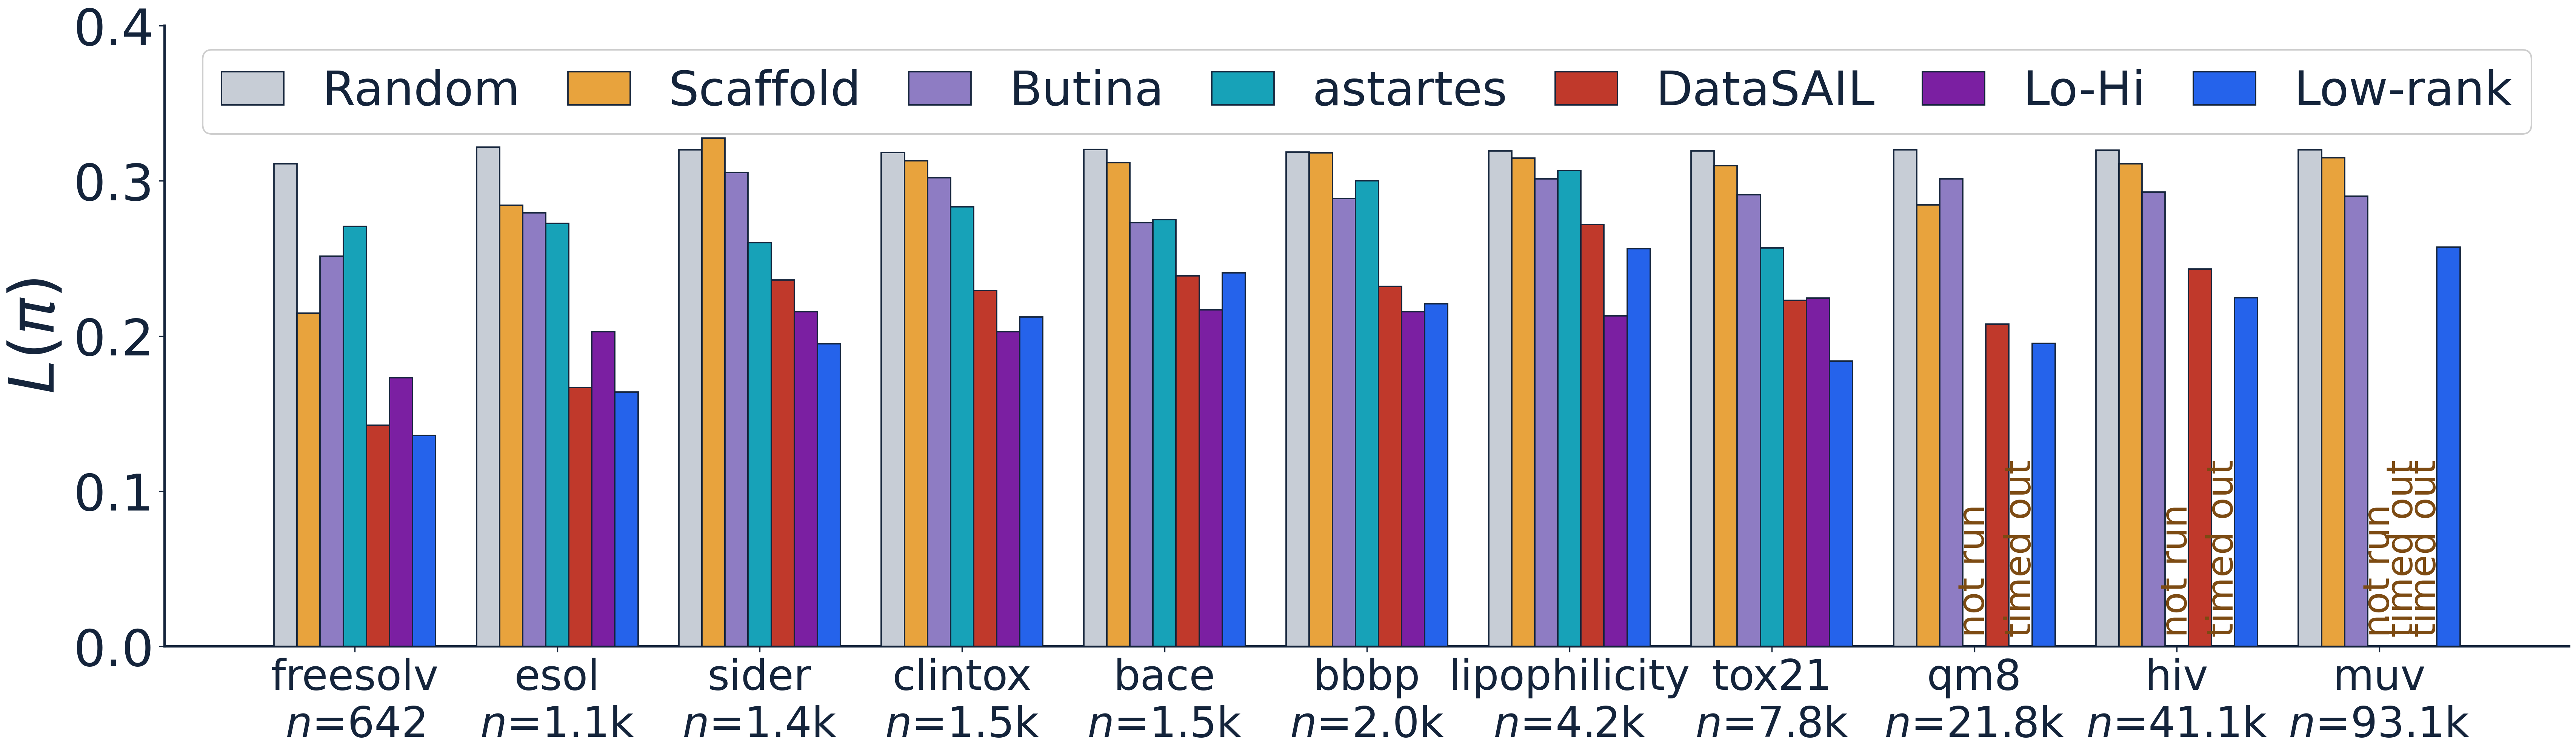
\includegraphics[width=\linewidth]{fig_moleculenet_leakage_vs_baselines}\end{center}
\vspace{-0.3ex}
{\centering\normalsize \textbf{Scaffold} sits at the random baseline on 8/11
(\emph{worse} than random on \emph{sider}); \textbf{Butina} clustering helps only
modestly. Only \emph{optimizing the leakage objective} drops well below random.\par}

\vspace{0.4ex}
{\large\textbf{(b) Fast where the exact methods are not.} Split time, log--log.
Low-rank splits 93k in \textbf{2.6\,s}; ILP/MILP sit 1--3 orders above.}
\begin{center}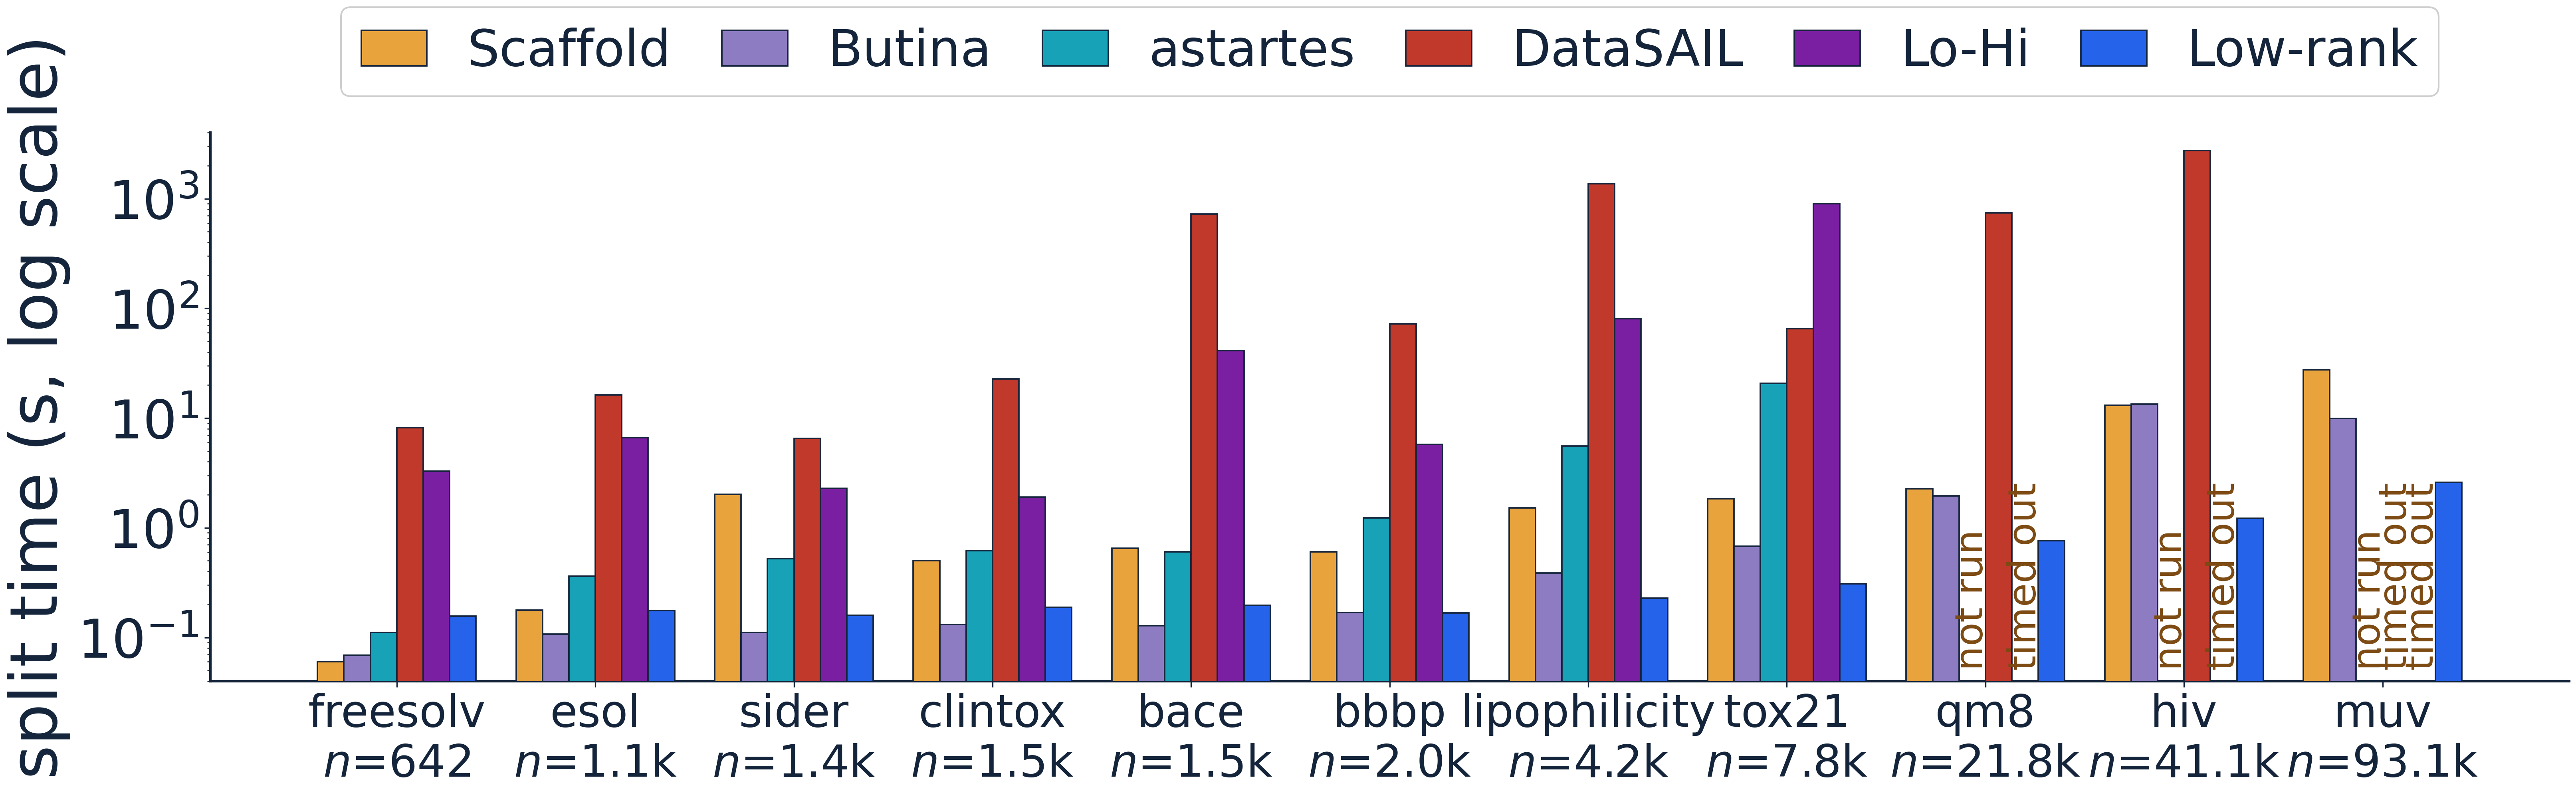
\includegraphics[width=0.66\linewidth]{fig_moleculenet_time_vs_baselines}\end{center}

\vspace{0.4ex}
{\large\textbf{(c) Vs.\ the two exact leakage-aware methods.}}
\begin{center}\setlength{\tabcolsep}{6pt}\renewcommand{\arraystretch}{1.35}
\normalsize
\begin{tabular}{l c c c}
\toprule
 & \textbf{DataSAIL} & \textbf{Lo-Hi} & \cellcolor{softblue}\textbf{Low-rank} \\
 & (ILP) & (MILP) & \cellcolor{softblue} \\
\midrule
Lower $L(\pi)$   & 1/10     & 0/8           & \cellcolor{softblue}\textbf{9/10,\ 8/8} \\
Split time       & $\le$90\,min & $\le$15\,min & \cellcolor{softblue}\textbf{$\le$27\,s} \\
Largest $n$ run  & 100k     & 7.8k          & \cellcolor{softblue}\textbf{9.55M} \\
Keeps all data   & yes      & \textbf{no}   & \cellcolor{softblue}yes \\
\bottomrule
\end{tabular}
\end{center}
\vspace{-0.3ex}
{\centering\small\emph{Scope:} neither can be forced to exact 80/20, so $L(\pi)$
is matched on each method's \emph{own} ratio — Lo-Hi on the subset it retains
(it discards 0.1–2\%). DataSAIL re-run locally; its only $L(\pi)$ win is
\emph{bace}. Time \& largest-$n$ include the OMol25 runs.\par}
\vspace{0.2ex}
{\centering\tiny Lo-Hi: Steshin, S.\ \emph{Lo-Hi: Practical ML Drug Discovery
Benchmark}.\ NeurIPS 2023 Datasets \& Benchmarks Track.\par}

\end{minipage}\hfill
%------------------------------- COLUMN 3 ----------------------------------
\begin{minipage}[t]{0.313\linewidth}

\pblock{Scaling to $10^7$: time \& leakage}
\begin{center}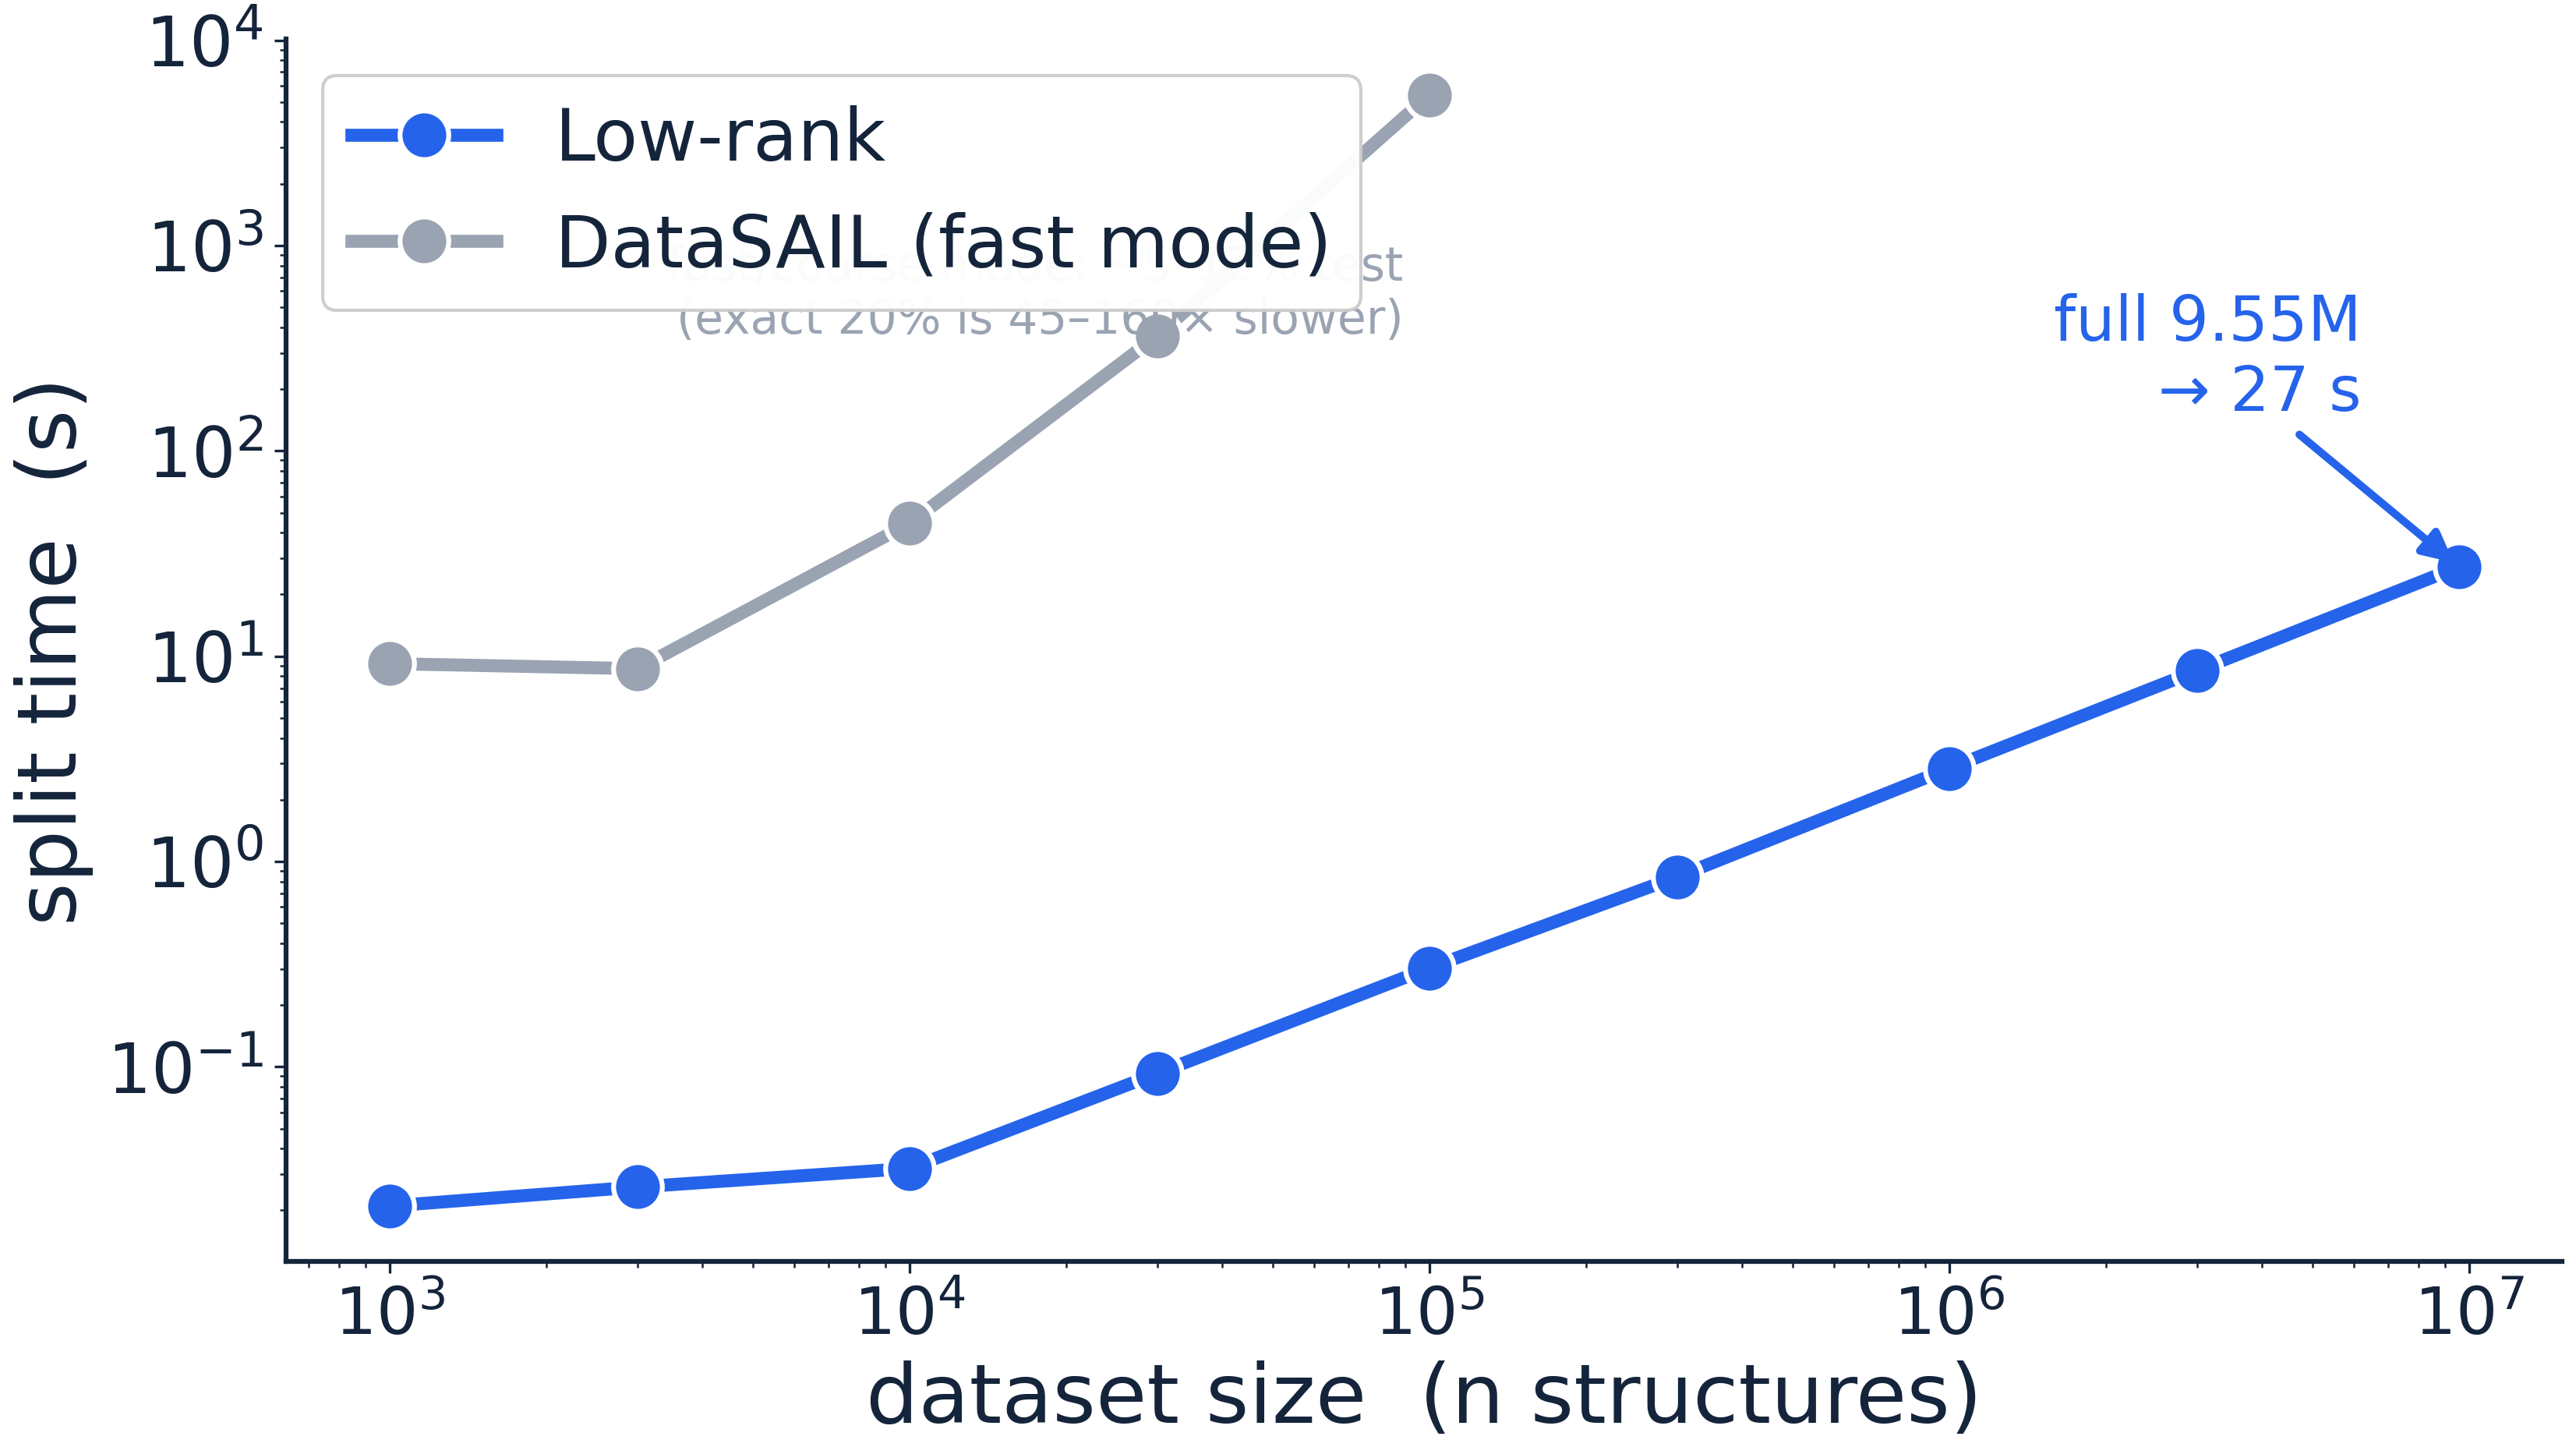
\includegraphics[width=0.47\linewidth]{fig_omol25_scaling_to_9-55M}\hfill%
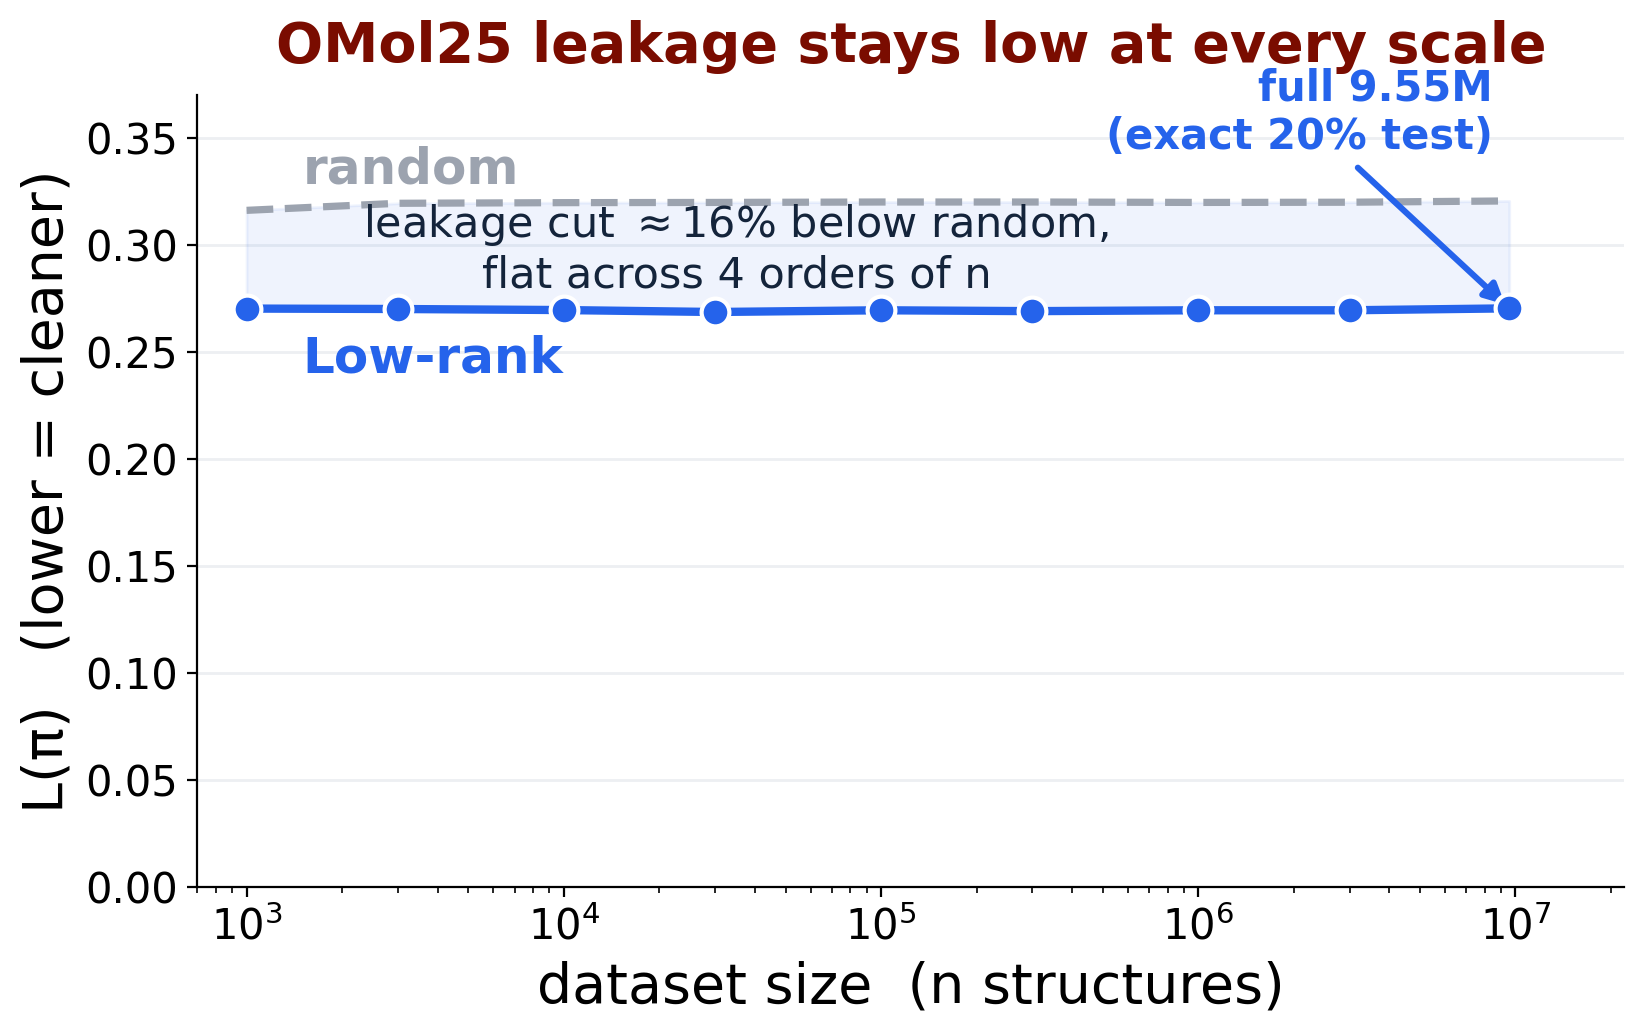
\includegraphics[width=0.45\linewidth]{fig_omol25_lpi}\end{center}
\vspace{-0.2ex}
{\centering\large \textbf{Left:} split time vs.\ $n$ (log–log). Low-rank traces a
straight $O(n\,r)$ line, splitting all \textbf{9.55M} structures in \textbf{27\,s};
DataSAIL, even in its \emph{fastest} mode, stalls at \textbf{90\,min} (100k) and is
\textbf{out-of-memory} by 300k. \textbf{Right:} $L(\pi)$ stays $\approx$16\% below
random and \textbf{flat} across four orders of $n$, at an \emph{exact} 20\% test
split.\par}

\pblock{Head-to-head with DataSAIL}
\callout{soft}{\centering\large \textbf{Embedding-agnostic:} it runs
\emph{directly} on OMol25's metal complexes and radicals. Scaffold, Butina \&
Lo-Hi need \textbf{SMILES} and \emph{cannot run} here at all.}
\vspace{0.4ex}
\begin{center}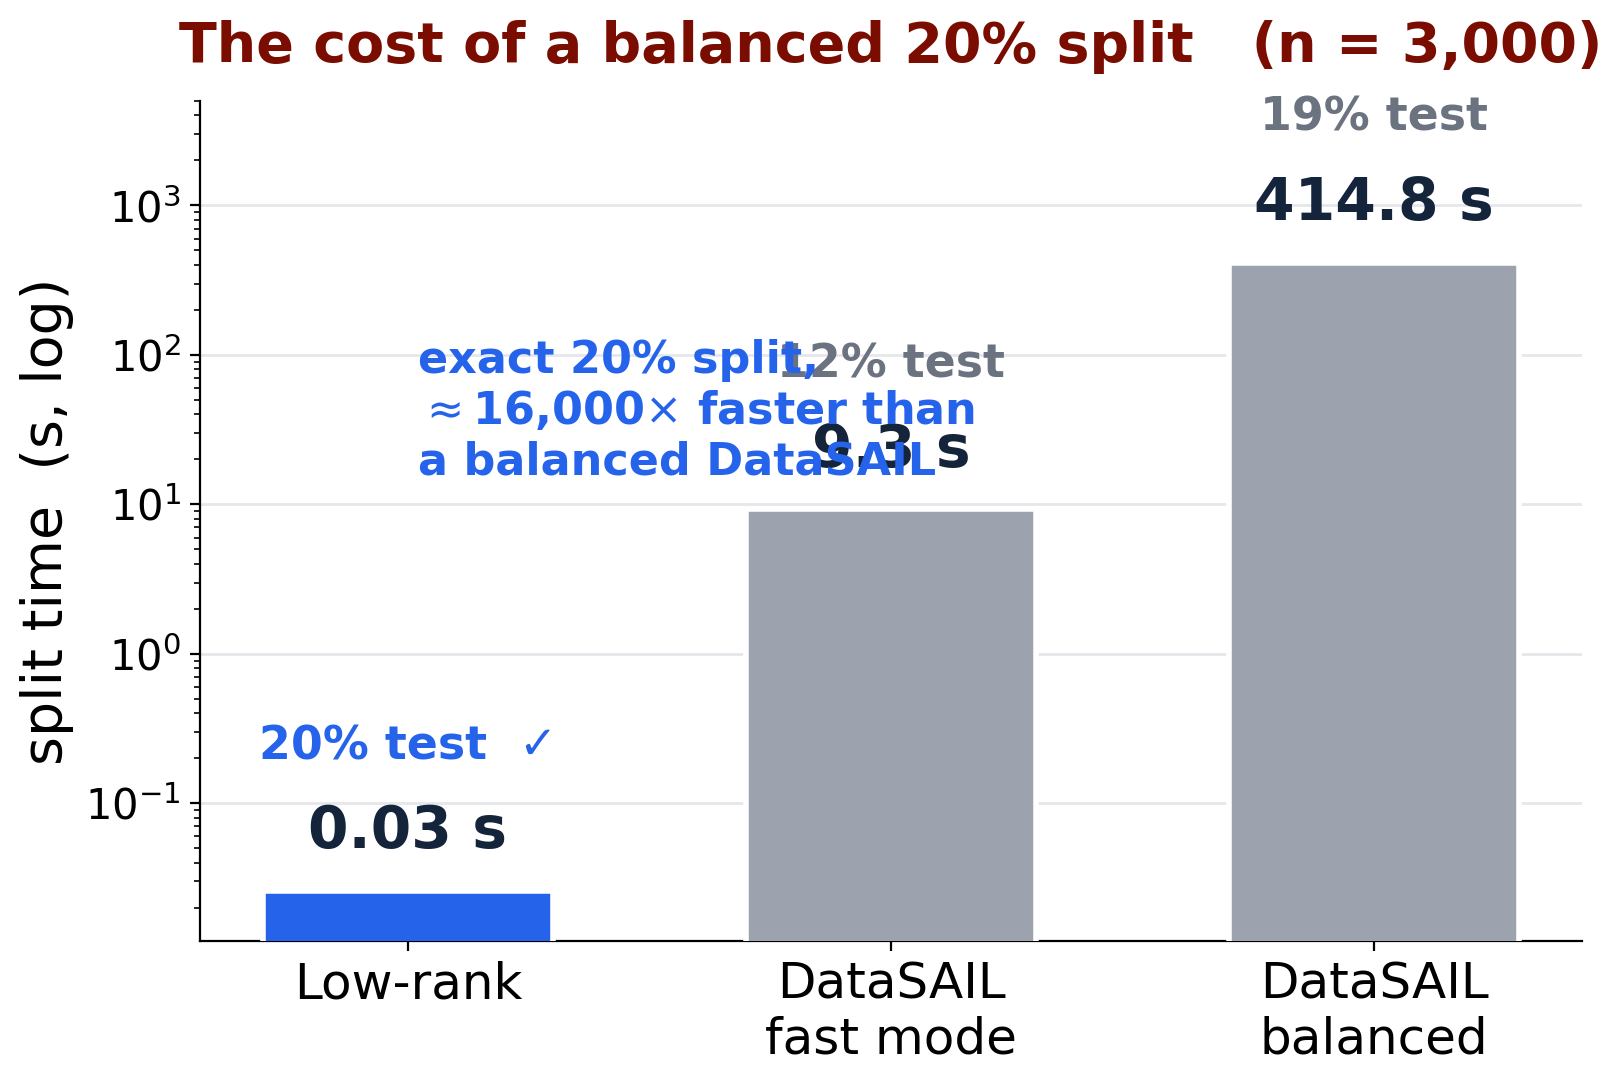
\includegraphics[width=0.60\linewidth]{fig_omol25_lpi_vs_datasail}\end{center}
\vspace{-0.3ex}
{\centering\large DataSAIL's \textbf{fast} mode collapses the test set to
\textbf{5–12\%} (never 20\%); forcing $\approx$20\% needs fine clustering that is
\textbf{45--160$\times$ slower} and \emph{still} plateaus at 19\%. Low-rank hits
\textbf{exact 20\% in 0.03\,s} and holds it to 9.55M.\par}

\pblock{Discussion}
\begin{itemize}\setlength\itemsep{1pt}\large
  \item \textbf{Factorize, don't truncate.} Scoring the \emph{whole} similarity
        in $O(nr)$ (no k-NN truncation, no ILP) gives the \textbf{lowest $L(\pi)$
        of the fast splitters} (11/11), deterministically, in seconds.
  \item \textbf{Scale, reach, exact balance.} First leakage-aware splitter
        \emph{we know of} to reach $10^7$ (9.55M in 27\,s) and the \textbf{only
        one that runs on OMol25}; DataSAIL holds 80/20 only at 45--160$\times$ the
        cost, while low-rank gives \textbf{exact 20\%} at lower leakage.
  \item \textbf{Honest scope.} On an independent fingerprint the margins are
        \emph{comparable}, not lower; downstream-error validation is future work.
\end{itemize}

\end{minipage}
\end{minipage}};
% --- vertical column separators (top just below header, down to footer) ---
\draw[rulec, line width=1.6pt]
   ([xshift=36.0cm, yshift=-15.9cm]current page.north west) --
   ([xshift=36.0cm, yshift=-84.6cm]current page.north west);
\draw[rulec, line width=1.6pt]
   ([xshift=70.7cm, yshift=-15.9cm]current page.north west) --
   ([xshift=70.7cm, yshift=-84.6cm]current page.north west);
\end{tikzpicture}

\end{frame}
\end{document}
